\section{Property Graph Matching Framework}\label{sec:framework}
\begin{figure}[ht]
  \centering
  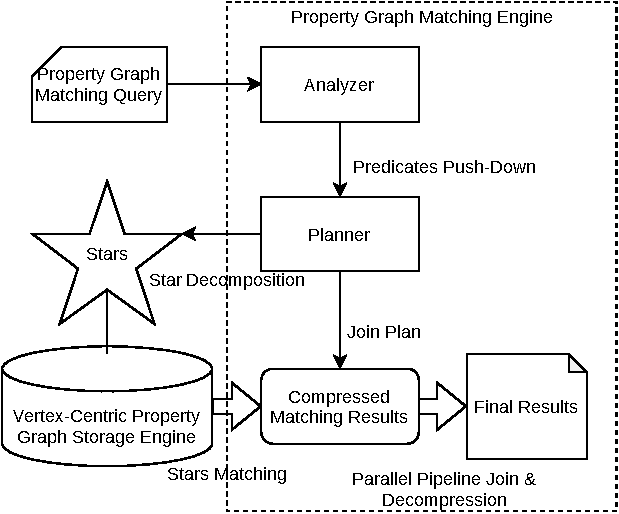
\includegraphics[width=0.48\textwidth]{img/architecture.pdf}
  \caption{The workflow of our property graph matching framework.}\label{img:architecture}
\end{figure}
Figure~\ref{img:architecture} shows the workflow of our property graph matching framework,
and Figure~\ref{img:pattern_graph} shows a popular diamond pattern in the field of recommendation system~\cite{DBLP:journals/pvldb/GuptaSGGZLL14,DBLP:journals/pvldb/SharmaJBLL16}.
Because of the complexity of the real-world property graphs,
the conventional in/out-edges storage method is not suitable and would incur many unnecessary random disk accesses,
and in Section~\ref{sec:storage}, we develop a vertex-centric property graph storage model to address the problem.
Based on the storage model, in Section~\ref{sec:match},
we propose a property graph matching engine that is able to solve real-world problems by leveraging the economical disk:
The core of the engine is the planner, which avoids random disk accesses by decomposing the pattern into a series of stars.
Compared with existing work, we take steps further by introducing
1\@. a matching-result compression algorithm which reduces the cost of materializing intermediate results;
and 2\@. a predicate push-down optimizer that is able to filter out unnecessary matchings in an early stage and reduce the burden of the join process.
We now describe our framework in more detail:
\begin{figure}[ht]
  \centering
  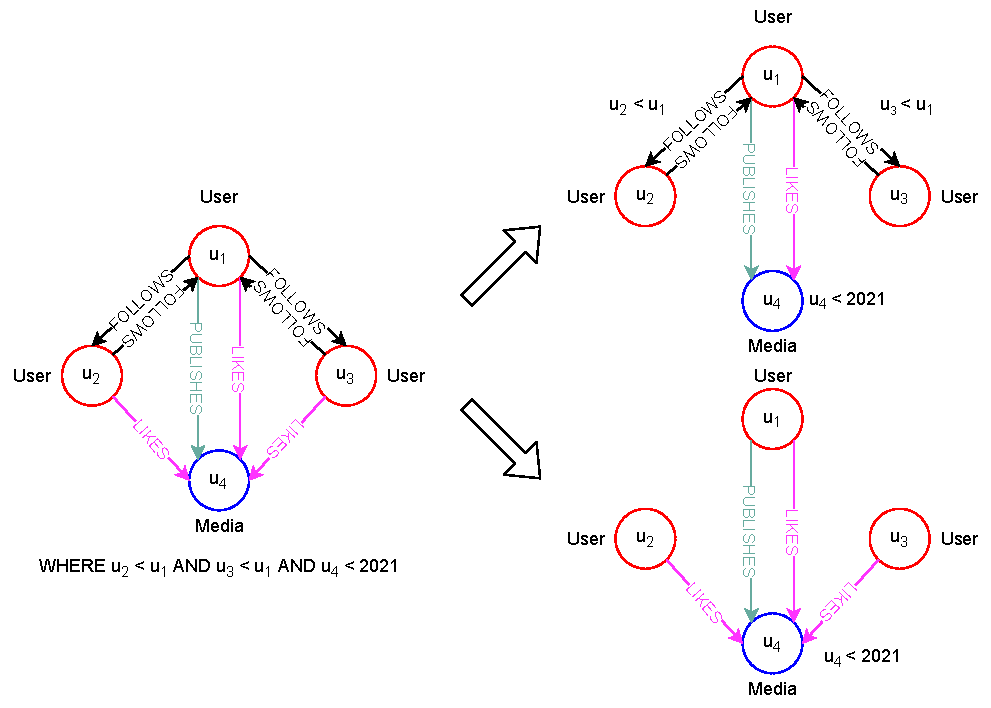
\includegraphics[width=0.48\textwidth]{img/pattern_graph.pdf}
  \caption{A pattern for recommendation system of social network and the decomposition of stars.}\label{img:pattern_graph}
\end{figure}

The vertex-centric storage engine is designed to be I/O efficient and support the real-world property graph well.
The conventional way to store graphs on disk is to store the in/out-edges separately for each vertex,
via the compressed sparse column (CSC) and the compressed sparse row (CSR) format~\cite{DBLP:conf/sc/PearceGA10}.
However, we find that the conventional graph store method has limitations for real-world property graph:
because of the existence of multi-edges,
one has to scan all the in/out-edges to check whether a vertex could be matched if the graph is stored in the traditional way, which is time consuming and I/O inefficient.
To address this problem, in Section~\ref{sec:storage},
we propose a vertex-centric storage model by storing all the necessary local information together with the neighbors,
such that all the unnecessary scanning are avoided.
Moreover, we develop two kind of simple indices to boost the searching of vertices, which reduces I/Os even further.

The property graph matching engine adopts a join-based method.
Generally speaking, there are two kinds of approaches to solve the graph isomorphism problem:
one is the tree-based searching algorithm~\cite{DBLP:journals/jacm/Ullmann76,DBLP:conf/sigmod/HanLL13}, and the other is the join-based method~\cite{DBLP:journals/pvldb/LaiQLC15,DBLP:journals/pvldb/QiaoZC17,DBLP:journals/pvldb/MhedhbiS19}.
Because of the poor locality of graphs, significant random disk reads may incur when implementing an out-of-core tree-based searching algorithm~\cite{DBLP:conf/sigmod/KimLBHLKJ16}, and thus we choose the join-based approach.
The most fundamental problem for a join-based algorithm is to choose the basic matching unit.
A straightforward approach is to match the edges of a pattern and then join on the edges' matching results,
however, incredible amount of useless intermediate results would be generated by doing so,
because an edge contains very little filtering information such as degrees and neighborhood structures.
Some authors address the problem by joining on more complex structures such as multi-hop edges or frequent subgraphs,
however, it is costly to pre-build proper indices and they require super-linear space~\cite{DBLP:journals/pvldb/SunWWSL12}.
Based on these observation, we make a trade-off by choose stars as our basic unit.
A star contains a root vertex and the neighbors of the root.
Thanks to our vertex-centric storage model, in Section~\ref{sec:match_star}, we'll show that we could scan the huge data graph at most once to obtain the stars' matching results, and all the disk accesses are sequential.
Some authors also use star-like structures as their join unit~\cite{DBLP:journals/pvldb/SunWWSL12,DBLP:journals/pvldb/LaiQLC15}, however, we take more steps further by improving the star decomposition algorithm to contain as much filtering information as possible, and our experiment shows that our algorithm could reduce the size of intermediate to $???\%$ and obtain $???\times$ speed-up.

For real-world billion node graphs, the intermediate result is another challenge that must be conquered.
Even though we could use stars to filter out many unnecessary matchings,
the intermediate results could still be gigantic for really huge graphs.
Moreover, the intermediate result grows exponentially with respect to the size of the data graph,
and they could be even larger than the original data graph.
Our experiment shows than a data graph with $???x$ edges may generate $???x$ ($???\times$) rows of matching results.
Most of the existing work rely on large physical memory to store the huge intermediate results,
which is financially expensive and limit the application of property graph matching.
To solve the challenge, in Section~\ref{sec:match_compress}, we design a very compact compression algorithm for stars' matching results.
By postponing the Cartesian product and digging the equivalence classes among the vertices in a star,
the compression ratio reaches as high as $10^{???}$ (Section~\ref{sec:experiments}).
And the compressed data is designed to be written sequentially such that we could write them to disk efficiently when memory is limited, i.e., solving a large property graph matching problem on a laptop.
Moreover, in Section~\ref{sec:match_join}, we propose a parallel pipeline join algorithm that is able to join directly on the compressed data, so the memory is saved.

A graph matching query consists two parts: the pattern graph description part (the MATCH clause) and the constraint specification part (the WHERE clause).
For example, Figure~\ref{img:cypher_query} shows the Cypher query (Neo4j's graph query language) corresponds to the pattern in Figure~\ref{img:pattern_graph}.
Existing graph matching frameworks usually neglect the WHERE clause,
because they could always be applied as filters after the graph isomorphism result is obtained.
However, the WHERE clause is ubiquitous in real-world property matching queries and they contains many user specified constraints~\cite{DBLP:journals/csur/AnglesABHRV17},
it is desirable to push them down to the graph isomorphism searching phase and make full use of these searching constraints when solving a real-world property graph matching problem.
However, it is still challenging to push down the predicates, because it depends on the graph matching algorithm and the predicates may involve in vertices not in a basic matching unit.
To address this problem, in Section~\ref{sec:match_optimize}, we propose a novel predicates splitting algorithm that is able to extract useful searching constraints from the WHERE clause and push them down to the star matching process,
which reduces the intermediate results in an early stage.
Our experiment shows that, we could save $???\%$ of the space if the WHERE clause is handled properly,
and the overall performance is $???\times$ better then the naive approach.
\begin{figure}[ht]
  \begin{verbatim}
    MATCH (u1:Person)-[:FOLLOWS]->(u2:Person)-[:FOLLOWS]->(u1),
          (u1)-[:FOLLOWS]->(u3:Person)-[:FOLLOWS]->(u1),
          (u1)-[:PUBLISHES]->(u4:Media), (u1)-[:LIKES]->(u4),
          (u2)-[:LIKES]->(u4)<-[:LIKES]-(u3)
    WHERE u1 < u2 AND u1 < u3 AND NOT (u2 >= u3 OR u4 >= 2020)
  \end{verbatim}
  \caption{Graph matching query of the pattern graph in Figure~\ref{img:pattern_graph}.}\label{img:cypher_query}
\end{figure}
